\documentclass{article}
\usepackage[landscape, bottom = 1cm, left=1cm, right=1cm]{geometry}
\usepackage{url}
\usepackage{multicol}
\usepackage{amsmath}
\usepackage{esint}
\usepackage{amsfonts}
\usepackage{tikz}
\usetikzlibrary{decorations.pathmorphing}
\usepackage{amsmath,amssymb}
\usepackage{pgfplots}
\usepackage{caption}
\usepackage{graphicx}
\usepackage{pifont}
\usepackage{colortbl}
\usepackage{xcolor}
\usepackage{mathtools}
\usepackage{amsmath,amssymb}
\usepackage{enumitem}
\makeatletter

\usepackage[english]{babel}
\usepackage[utf8]{inputenc}

\advance\topmargin-.5in
\setlength{\parindent}{0pt}
%\advance\textheight3in
%\advance\textwidth1in

\begin{document}
	\begin{multicols*}{2}
	\begin{center}
		{\huge{\textbf{Reinforcement Learning Cheat Sheet}}}
	\end{center}
	\section*{Notation}
		To help understand different concepts, we use symbol  \ding{56} to indicate the difficulty of the materials. \ding{56} means simple, \ding{56}\ding{56} means the materials might require several read to understand, and \ding{56}\ding{56}\ding{56} is simply dangerous. \\
		
		In general, random variables are upper case and the values of the random variable are lower case. Matrices are bold. \\
		
		\begin{tabular}{lp{5cm} l}
		Symbol   & Meaning \\
		$t$ & a discrete time\\
		$S_t$ & state at time t \\
		$A_t$ & action at time t \\
		$R_t$ & reward at time t \\
		$\mathcal{S}$ & set of all non-terminal states \\
		$ \mathcal{A}$ & set of all actions \\
		$ \mathcal{R}$ & set of all rewards \\
		$ \doteq $ & definition equal 
		\end{tabular}

		\section*{Problem setup: Markov decision processes}
		\begin{center}
		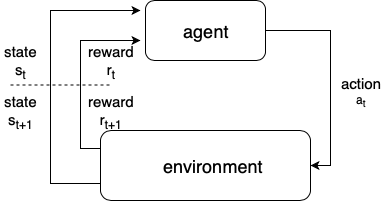
\includegraphics[width=6cm]{../img/env.png}
		\captionof{figure}{Actor-critic relation}
		\label{plot:env}
		\end{center}
		
		\ding{56} In a Markov decision process (MDP) shown in Figure \ref{plot:env}, a game agent interacts with an environment to achieve a certain goal. The interaction happens at every discrete time $ t = 1, 2, 3, ... $. The agent observes certain state of the environment $ S_t \in \mathcal{S} $, selects some action $ A_t \in \mathcal{A} $ and then receives certain reward $ R_{t+1} \in \mathcal{R} $. In a finite MDP, $ p(s', r|s, a) = Pr\{S_t=s', R_t=r | S_{t-1}=s, A_{t-1}=a \} $. The expected reward can be computed by $ r(s, a) = \mathbb{E}[R_t |S_{t-1} = s,A_{t-1}=a] = \sum_{r \in \mathcal{R}}r \sum_{s' \in \mathcal{S}} p(s', r | s, a) $.  \\
		
		The goal of a game is typically to maximize the return. The discounted reward can be framed by:
		\begin{align*}
			 G_t \doteq R_{t} + \gamma R_{t+1} + \gamma^{2}R_{t+2} + ... \doteq  \sum_{k=0}^{\infty} \gamma^{k}R_{t+k} 
		\end{align*}
		$ \gamma \in [0, 1] $ is the discount factor.
		
		\section*{Policy gradient}
			\ding{56} Different from value-based methods which estimate the state-action or value-state function, policy gradient tries to find out the best policy to follow. The policy function $ \pi(a | s) \doteq Pr\{A_t = a | S_t = s, \theta_t = \theta \} $ where $ \theta$ is the fuction parameter. The optimizatino of the function parameter can be described as 
		\begin{equation}\label{eq:policyg}
		\theta_{t+1} = \theta_t + \alpha \nabla_\theta J(\theta) 
		\end{equation}
		
		Here we try to do an ascent by setting $ J(\theta) = V_\pi(s_0) $, which means that we try trying to maximize the state value of the initial state under policy $ \pi $. Here we introduce the policy gradient theorem which we will use to do the update in equation \ref{eq:policyg}.
		\paragraph{\ding{56}\ding{56} Policy gradient theorem}
		The policy gradient theorem states that:
		$$ \nabla_\theta J(\theta) \propto \sum_{s \in \mathcal{S}} \mu_\pi (s) \sum_{a \ \in \mathcal{A}} q_\pi (s,a) \nabla_\theta \pi_\theta(a | s) $$
		$ \mu_\pi (s) $ is the time that the agent spends in state $ s $ under policy $ \pi$. The prove is provided below:
		\begin{align*}
		{}& \nabla_\theta J(\theta)  = \nabla_\theta V_\pi (s_0)   \\
		={}& \nabla [ \sum_a q_\pi(s, a) \pi(a | s, \theta) ] \\
		={}& \sum_ a [ \nabla \pi(a | s, \theta) q_\pi(s, a) +  \pi(a | s, \theta)  \nabla  q_\pi(s, a)] \text{ (product rule)} \\
		={}& \sum_ a [ \nabla \pi(a | s, \theta) q_\pi(s, a) + \pi(a | s, \theta) 
		\nabla  \sum_{s', r'} p(s', r' | s, a) (r' + V_\pi(s')) ]  \\
		={}& \sum_ a [ \nabla \pi(a | s, \theta) q_\pi(s, a) + \pi(a | s, \theta)  
		+  \sum_{s', r'} p(s', r' | s, a)  \nabla  V_\pi(s') ] \\
		={}& \sum_ a [ \nabla \pi(a | s, \theta) q_\pi(s, a) + \pi(a | s, \theta)  
		 +  \sum_{s'} p(s' | s, a) \nabla  V_\pi(s') ] \\
		{}&( \text{because} \sum_{s'} p(s' | s, a) = \sum_{s', r'} p(s', r' | s, a) ) 
		\end{align*} 
		
		If we keep expanding the gradient on $ V_\pi(s'), V_\pi(s''), ... $, we will have  
		a recursive definition which is equivalent to $ \sum_{s \in \mathcal{S}} \sum_{k=0}^\infty p(s, x, k)  \sum_ a \nabla \pi(a | s, \theta) q_\pi(s, a) $ where 
		$ p(s, x, k) $ denotes the probability to go from state $ s $ to state $ x $ in $ k $ steps. 
		
		\section*{Actor-critic}
		\begin{center}
		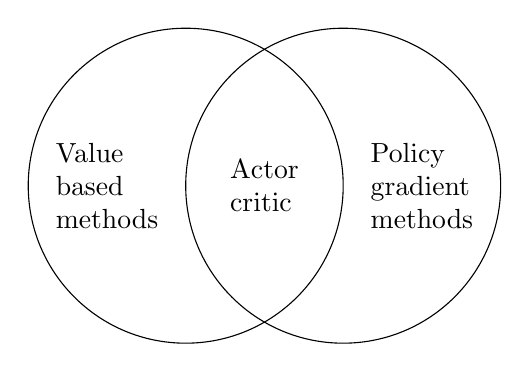
\begin{tikzpicture}
		\draw (2.0, 2) node[align=left] {Value \\  based \\ methods};
		\draw (4.0, 2) node[align=left] {Actor \\ critic};
		\draw (6.0, 2) node[align=left] {Policy \\  gradient \\ methods};
		\draw (3,2) circle (2.0cm) ;
		\draw (5,2) circle (2.0cm);
		\end{tikzpicture}
		\captionof{figure}{Actor-critic relation}
		\label{plot:ac}
		\end{center}
		
		\ding{56} Actor-critic  (AC) methods lay between value-based and policy gradient methods as shown in figure \ref{plot:ac}. They both estimate the policy and state-action functions, whereas value-based methods only estimate state-value functions and have an implicit $\epsilon$-greedy policy, and policy gradient methods do not have value function and only estimates the policy.
		
		\section*{Deep Q-learning (DQN)}
					\ding{56} DQN sits on the basis of many deep RL techniques. It tries to use a deep neural network to estimate the Q-value instead of using a linear method which has been proven to be more effective. The opitmal Q-value should tell us the max reward one can have by taking certain action: $ Q^*(s, a) = \mathbb{E}_{\pi} [G_t | S_t=s, A_t=a ] $. The Bellman equation describes that $ Q^*(s, a) = \mathbb{E}_{\pi} [R_t + \gamma \max_{a'} Q^*(s', a' | s, a)] $.  \\
		
		Given a neural network with parameter $ \theta $, and the target Q-value $ R_t + \gamma \max_{a'} Q^*(s', a' | s, a) $ the update gradient on the loss function can be defined as: 
		\begin{equation*}
		\begin{split}
		\nabla_{\theta^-}L(\theta) =  &  \mathbb{E}[(R_t + \gamma \max_{a'}\\
		&Q(s', a' | \theta^-) - Q(s, a | \theta)) \nabla Q(s, a | \theta) ] 
		\end{split}
		\end{equation*}
		where $ \theta^-$ is the old network parameter used to estimate the target value. Futhuremore, DQN also incoprates two other techniques to improve the performance, namely experience replay and using a second network  to generate the target Q value. 
		
		The benefits of experience replay:
		\begin{itemize}
		\item More data efficiency as one sample might get used more than once.
		\item Using consecutive samples might not be efficient as consecutive samples might be highly correlated which means that they contain overlapping information. For example, during gameplay, if an agent is in the left half of the environment, the consecutive plays are more likely in the left half as well which might contain overlapping information.
		\item To make learning sample distribution independent of model parameters. On-policy learning might bias the probability of sample distribution. For instance, if the model thinks the action to move left is greater, then all the states will have greater probabilities of being reached and vice versa. It is easy to see how an agent can get stuck in a local minimum while oscillating between left and right.
		\end{itemize}
		
		Using two networks for the Q value is to reduce variance. When learning, if $ Q(s_{t}, a) $ increases, often $ Q(s_{t+1}, a), \forall a \in \mathcal{A} $ increases, which could lead to divergence.
		
	\end{multicols*}
\end{document}


